\documentclass[twoside,openright,final]{bhamthesis}
\usepackage[utf8]{inputenc}
\usepackage{amssymb}
\usepackage{amsmath}
\usepackage{listings}
\usepackage{geometry}
\usepackage{indentfirst}
\usepackage{graphicx}
\graphicspath{ {images/} }
\usepackage{enumerate,letltxmacro}
\usepackage{enumitem}
\LetLtxMacro\itemold\item
\renewcommand{\item}{\itemindent0.5cm\itemold}
\usepackage{hyperref}
\hypersetup{
    colorlinks,
    citecolor=black,
    filecolor=black,
    linkcolor=black,
    urlcolor=black
}
\usepackage{etoolbox}
\patchcmd{\thebibliography}{\section*{\refname}}{}{}{}
\pagestyle{plain}

\newcommand*{\approxident}{%
  \mathrel{\vcenter{\offinterlineskip
  \hbox{$\sim$}\vskip-.35ex\hbox{$\sim$}\vskip-.35ex\hbox{$\sim$}}}}

\usepackage{cite}

\setlength{\oddsidemargin}{1cm} % 2cm margin on the left for odd pages
\setlength{\evensidemargin}{0cm} % 2cm margin on the right for even pages

\title{\textbf{Parsing Regular Expressions in Agda}}
\department{Computer Science}
\degree{BSc. Computer Science}
\author{Wai Tak, Cheung}
\studentid{1465388}
\supervisor{Dr. Martín Escardó}

\begin{document}
\maketitle

\abstract
\par Blah blah blah. Blah blah blah. Blah blah blah. Blah blah blah. Blah
blah blah. Blah blah blah. Blah blah blah. Blah blah blah.
Blah blah blah. Blah blah blah. Blah blah blah. Blah blah blah. Blah
blah blah.
Blah blah blah. Blah blah blah. Blah blah blah. Blah blah blah.
Blah blah blah. Blah blah blah. Blah blah blah. Blah blah blah. \\ \\
Keywords: language, regular expression, finite automata, agda,
thompson's construction, powerset construction, proofs

\acknowledgments
\par Blah blah blah. Blah blah blah. Blah blah blah. Blah blah blah. Blah
blah blah. Blah blah blah. Blah blah blah.
Blah blah blah. Blah blah blah. Blah blah blah.
Blah blah blah. Blah blah blah. Blah blah blah. Blah blah blah. Blah
blah blah. Blah blah blah. Blah blah blah.
Blah blah blah. Blah blah blah. Blah blah blah. Blah blah blah. Blah
blah blah. Blah blah blah.
Blah blah blah. Blah blah blah. Blah blah blah. Blah blah blah. Blah
blah blah.

\repository
\vspace{7cm}
\begin{center}
  All software for this project can be found at \\
  https://codex.cs.bham.ac.uk/svn/projects/2015/wtc488/
\end{center}

\newpage
\section*{List of Abbreviations}
\addcontentsline{toc}{section}{List of Abbreviations}
\begin{tabular}{ll}
  \textbf{\(\epsilon\)-NFA} & Non-deterministic Finite Automaton with
                              \(\epsilon\)-transition \\
  \textbf{NFA} & Non-deterministic Finite Automaton \\
  \textbf{DFA} & Deterministic Finite Automaton \\
  \textbf{MDFA} & Minimised Deterministic Finite Automaton
\end{tabular}
\newpage

\newpage
\setcounter{tocdepth}{3}
\tableofcontents
\newpage

\section{Introduction}
\paragraph{} This project aims to study the feasibility of formalising
Automata Theory \cite{aho1972} in Type Theory with the aid of a dependently-typed
functional programming language, Agda \cite{agdawiki2016}. Automata
Theory is an extensive work; therefore, it will be unrealistic to include all
materials under the time constraint. Accordingly, this project will only focus on the theorems and
proofs that are related to the translation between regular expressions
and finite automata. Futhermore, this project also gives a brief introduction
on how complex and non-trival proofs are formalised in Type Theory. 

\paragraph{} The Agda formalisation can be separated into two major
components: 1) the translation from regular expressions to DFA and 2)
the correctness proofs of the translation. In this stage, we are only
interested in the correctness of the translation but not the efficiency. 

\subsection{Motivation}
\paragraph{} My motivation on this project is to learn and apply
dependent types in programming and in writing proofs. ...


\subsection{Overview}
\paragraph{} In section two, we will first give a brief introduction on
Agda as a programming language and as a proof assistant. Then we will
define the types that are frequently used in the project. We
will also look into some small Agda proofs so that readers can
have a taste of how proofs are formalised in Type Theory. In the end
of section two, we will discuss a similar reseach \cite{firsov2013}
conducted by Firsov and Uustalu. Following the
background, the third section will be a detail description of our
work. We will walk through the Agda
formalisation of the two components stated in previous part. After
that, we will introduce some possible extensions to the project. Then,
there will an evaluation. Finally, the conclusions will be drawn. 

\newpage
\section{Background}

\subsection{Agda} 
\paragraph{} Agda is a dependently typed functional programming language and a
proof assistant based on Intuitionistic Type Theory
\cite{martin1984}. The current version (Agda 2) is rewritten by Norell
\cite{norell2007} at the Chalmers University of
Technology. In this section, we will describe the basic features of
Agda and how dependent types are employed to build programs and
proofs. Most of the materials presented below can also be
found in the two tutorial papers \cite{bove2009} and
\cite{norell2009}. Interested readers can take a look at them and get
a more precise idea on how to work with Agda. We will begin by showing how to do ordinary
functional programming in Agda. 

\subsubsection{Simply Typed Functional Programming}
\paragraph{} Haskell is the implementaion language
of Agda, as we will see below, Agda has borrowed many features from
Haskell. In below, we will show how to define basic data types
(boolean and natural number) and functions over them. 

\paragraph{Boolean} We first introduce the type of boolean values in
Agda.  
\begin{lstlisting}[mathescape=true,xleftmargin=.3\textwidth]
data Bool : Set where
  true  : Bool
  false : Bool
\end{lstlisting}

\paragraph{} \(Bool\) is a data type which has two
constructors: \(true\) and \(false\). Note that these two constructors
are also elements of \(Bool\) since they take no argument. Their types are explicitly declared in '\(:
Bool\)'. On the other hand, \(Bool\) is a member of the type \(Set\). \(Set\)
represents the set of all \textit{small types}. \(Bool\) is a
\textit{small type} but \(Set\) itself is not, it is a \textit{large
  type}. We will look into the difference in later
part. Now, let us define the negation function on boolean values:
\begin{lstlisting}[mathescape=true,xleftmargin=.3\textwidth]
not : Bool $\to$ Bool
not true  = false
not false = true
\end{lstlisting}

\paragraph{} Unlike Haskell, we must provide a type declaration for every
functions. Note that we can declare partial
functions in Haskell but not in Agda. For instance, the function below
will be rejected by the Agda compiler:
\begin{lstlisting}[mathescape=true,xleftmargin=.3\textwidth]
not : Bool $\to$ Bool
not true  = false
\end{lstlisting}

\paragraph{Natural Number} The type of natural numbers is defined
inductively as follow: 
\begin{lstlisting}[mathescape=true,xleftmargin=.3\textwidth]
data $\mathbb N$ : Set where
  zero : $\mathbb N$
  suc  : $\mathbb N$ $\to$ $\mathbb N$
\end{lstlisting} 

\paragraph{} The constructor \(suc\) represents the successor of a given
natural number. For instance, \(1\) is represented as \(suc\
zero\). Now, let us define the addition over natural numbers as follow:
\begin{lstlisting}[mathescape=true,xleftmargin=.3\textwidth]
_+_ : $\mathbb N$ $\to$ $\mathbb N$ $\to$ $\mathbb N$: Set where
zero  + m = m
suc n + m = suc (n + m)
\end{lstlisting} 

\paragraph{Parameterised Types} In Haskell, the type of list \([a]\) is parameterised by the type
parameter \(a\). The analogus data type in Agda is defined inductively as:
\begin{lstlisting}[mathescape=true,xleftmargin=.3\textwidth]
data List (A : Set) : Set where
  []   : List A
  _::_ : A $\to$ List A $\to$ List A
\end{lstlisting} 

\subsubsection{Universe}
\paragraph{} ...

\subsubsection{Dependent Types}
\paragraph{} Dependent types are types that depend on values of other
types. For example, \(A^n\) is the type of vectors with
length \(n\) (depends on \(n\)). These kinds of types are not possible
to be declared in simply-typed systems like Haskell or Ocaml. Now, let
us look at how it is defined using dependent type in Agda. 
\begin{lstlisting}[mathescape=true,xleftmargin=.25\textwidth]
data Vec (A : Set) : $\mathbb N$ $\to$ Set where
  []   : Vec A zero
  _::_ : $\forall$ {n} $\to$ A $\to$ Vec A n $\to$ Vec A (suc n)
\end{lstlisting} 

\paragraph{} In the type declaration \(data\ Vec\ (A : Set) :\ \mathbb N \to
Set\ where\), \(A : Set\) is a type parameter defining the type of
elements in the vector. While the part \(\mathbb N \to Set\) means
that \(Vec\) takes a value \(n\) of type \(\mathbb N\) and produce a
vector type of A that depends on \(n\). For example, \(Vec\ A\ zero\) is the type of vectors with
zero length. 

\paragraph{} With dependent types, we can define data types and
functions which are more expressive and precise. For instance, we can
define the function \(head\) which returns the first element in a
vector as follow:
\begin{lstlisting}[mathescape=true,xleftmargin=.25\textwidth]
head : {A : Set}{n : $\mathbb N$} $\to$ Vec A (suc n) $\to$ A
head (x :: xs) = x 
\end{lstlisting} 
\paragraph{} Unlike in Haskell which we need to pattern match on \([]\)
and produce an error, we only need to pattern match on the case (\(x :: xs\)) here
because the type \(Vec\ A\ (suc\ n)\) ensures that the argument will never
be \([]\). Apart from vectors, we can also define the type of binary
search tree such that the order of elements in the tree is guranteed by
the type declaration. However, we will not be looking into that as it
is not our major concern. Interersted readers can take a look at
Section 6 in \cite{bove2009}. Other than data type declaration,
dependent types are also used to encode predicate logic and
program specifications. We will look at these two applications in
later parts in this section. 

\subsubsection{Propositions as Types}
\paragraph{} In the 1930s, Curry identified the
correspondence between propositions in propositional logic and types
\cite{curry1934}. After that, in the 1960s, de Bruijn and Howard extended
Curry's correspondence to predicate logic by introducing dependent
types \cite{bruijn1968, howard1969}. Later on, Martin-Lof published
his work, Intuitionistic Type Theory \cite{martin1984}, which turned the correspondence into a new
foundational system for constructive mathematics. 

\paragraph{} In the paragraphs below, we will show how the correspondence is
formalised in Agda. Note that the Intuitionistic Type
Theory is based on constructive logic; therefore, in this project, we
are working with constructive logic rather than classical logic. Interested readers can take a look at
\cite{avigad2000}. 

\paragraph{Propositional Logic} In general, Curry's correspondence
states that a proposition can be interpreted as a set of its proofs. A
proposition is true if and only if its set of proofs is inhabited,
i.e. there is at least an element in the set; it is false if and only
if its set is empty. 

\subparagraph{Truth} For a proposition to be true, the corresponding
type must have at least one element. 
\begin{lstlisting}[mathescape=true,xleftmargin=.3\textwidth]
data $\top$ : Set where
  tt : $\top$
\end{lstlisting} 

\subparagraph{Falsehood} For a proposition to be false, the corresponding
type must have no element at all. 
\begin{lstlisting}[mathescape=true,xleftmargin=.3\textwidth]
data $\bot$ : Set where
\end{lstlisting} 

\subparagraph{Conjunction} Suppose \(A\) and \(B\) are propositions, then the
proofs of \(A \wedge B\) should be consist of
a proof of \(A\) and a proof of \(B\). In Type Theory, it corresponds
to the product type. 
\begin{lstlisting}[mathescape=true,xleftmargin=.3\textwidth]
data _$\times$_ (A B : Set) : Set where
  _,_ : A $\to$ B $\to$ A $\times$ B
\end{lstlisting} 

\paragraph{} The above construction corresponds to the introduction rule of
conjunction while the elimination rules correspond to the functions
\(fst\) and \(snd\):
\begin{lstlisting}[mathescape=true,xleftmargin=.3\textwidth]
fst : {A B : Set} $\to$ A $\times$ B $\to$ A
fst (a , b) = a

snd : {A B : Set} $\to$ A $\times$ B $\to$ B
snd (a , b) = b
\end{lstlisting} 

\subparagraph{Disjunction} Suppose \(A\) and \(B\) are propositions, then the
proofs of \(A \vee B\) should be consist of either a proof of \(A\) or a
proof of \(B\). In Type Theory, it corresponds
to the sum type. 
\begin{lstlisting}[mathescape=true,xleftmargin=.3\textwidth]
data _$\uplus$_ (A B : Set) : Set where
  inj$_1$ : A $\to$ A $\uplus$ B
  inj$_2$ : B $\to$ A $\uplus$ B
\end{lstlisting} 

\paragraph{} Here is the function corresponds to the elimination rule of
disjunction:
\begin{lstlisting}[mathescape=true,xleftmargin=.2\textwidth]
$\uplus$-elim : {A B C : Set} $\to$ A $\uplus$ B $\to$ (A $\to$ C) $\to$ (B $\to$ C) $\to$ C
$\uplus$-elim (inj$_1$ a) f g = f a
$\uplus$-elim (inj$_2$ b) f g = g b
\end{lstlisting} 

\subparagraph{Negation} Suppose \(A\) is a proposition, then negation is
defined as a function that transform any arbitary proof in \(A\) to
the falsehood. It is defined as follow: 
\begin{lstlisting}[mathescape=true,xleftmargin=.3\textwidth]
$\neg$ : Set $\to$ Set
$\neg$ A = A $\to$ $\bot$
\end{lstlisting} 

\subparagraph{Implication} Suppose \(A\) and \(B\) are propositions,
we say that \(A\) implies \(B\) if and only if we can
transform any arbitary proof of \(A\) into a proof of \(B\). In Type
Theory, it corresponds to a function from \(A\) to \(B\), i.e. \(A \to
B\). 

\paragraph{Predicate Logic} We will now move to predicate logic and
introduce the universal (\(\forall\)) and existenial (\(\exists\)) quantifiers. 

\subparagraph{Universal Quantifier} The interpretaion of the universal quantifier is similar to
implication. In order for \(\forall x\in A. B(x)\) to be true, we will have
to transform every proofs \(a\) of \(A\) to a proof of the proposition
\(B[x:=a]\). In Type Theory, it is represented by the function \((x :
A) \to B\ x\). 

\subparagraph{Existential Quantifier} ...

\paragraph{Propositional Equality} ... 

\subsubsection{Encoding Program Specifications}
\paragraph{} ...

\subsection{Related Work}
\paragraph{} Certified Parsing of Regular Languages. 


\newpage
\section{Formalisation in Type Theory}
\paragraph{} Let us recall the two components of the formalisation: 1) translating any
regular expressions to a DFA and 2) proving the correctness of the
translation. 

\paragraph{} In part 1), the translation was divided into the following steps. First, we
followed Thompson's construction algorithm to convert any regular expressions to an
\(\epsilon\)-NFA. Then we removed all the \(\epsilon\)-transitions in
the \(\epsilon\)-NFA by computing the \(\epsilon\)-closure for every states. After that, we used powerset
construction to create a DFA. Finally, we removed all the unreachable
states and then used quotient construction to obtain the minimised
DFA. 

\paragraph{} In part 2), the correctness proos of the above
translation were also separated into different steps according to part
1). For each of the translation steps in part 1), we proved
that the language accepted by the input is equal to the language
accepted by its translated output. i.e. \(L(regex) =
L(translated\ \epsilon\)-NFA\() = L(translated\) DFA\() =
L(translated\) MDFA\()\). 

\paragraph{} In the following parts, we will walk through the formalisation of
each of the above steps together with their correctness proofs. Note
that all the definitions, theorems, lemmas and proofs wriiten in below
are adapted to the formalisation in Agda. Now, before we go into
regular expressions and automata, we first need to have a
representation of subsets and languages as they are fundamental
elements in the theory. 

\subsection{Subsets and Decidable Subsets}

\paragraph{Definition 1.1} Suppose \(A\) is a set, in Type Theory, its
subsets are represented as a unary function on
\(A\), i.e. \(Subset\ A = A \to Set\). 

\paragraph{} When declaring a subset in Agda, we can write \(SubA =
\lambda\ a \to\ ?\), the \(?\) here defines the
condition for \(a\) to be included in \(SubA\). This construction is
very similar to set comprehension. For example, the subset 
\(\{a\ | \ a \in A,\ P(a)\}\) corresponds to \(\lambda\ a \to P\
a\). Subset is also a unary predicate of \(A\); therefore, the decidability of it will remain
unknown until it is proved. 

\paragraph{Definition 1.2} The other representation of subset is \(DecSubset\ A = A \to
Bool\). Unlike \(Subset\), its decidability is ensured by its
definition. 

\paragraph{} The two definitions have different purposes. \(Subset\) is used to represent \(Language\) because not every
language is decidable. For other parts 
such as a subset of states in an automaton, \(DecSubset\) is used
as the decidability is assumed in the definition. The two definitions
are defined in Subset.agda and Subset/DecidableSubset.agda
respectively as stated at the top. Operators such as membership (\(\in\)), subset
(\(\subseteq\)), superset (\(\supseteq\)) and equality (\(=\)) can
also be found in the two files. 

\paragraph{} Now, by using the representation of subset, we can define languages, regular expressions and finite
automata. 

\subsection{Languages}

\paragraph{} Suppose we have a set of alphabets \(\Sigma\); in Type Theory, it
can be represented as a data type, i.e. \(\Sigma : Set\). Notice that the decidable equality of
\(\Sigma\) is assumed. In Agda, they are passed to every modules as
parameters \((\Sigma : Set)\) \((dec : DecEq\ \Sigma)\). 

\paragraph{Definition 2.1} We first define \(\Sigma^*\) as the set of all
strings over \(\Sigma\). In our approach, it was expressed as a list of
\(\Sigma\), i.e. \(\Sigma^* = List\ \Sigma\). 

\paragraph{} For example, (\(A :: g ::
d :: a :: []\)) represents the string 'Agda' and the empty list \([]\)
represents the empty string \(\epsilon\). In this way, we can pattern
match on the input string in order to get the first
input alphabet and to run a transition from a particular state to another state. 

\paragraph{Definition 2.2} A language is a subset of 
\(\Sigma^*\); in Type Theory, \(Language = Subset\ \Sigma^*\). 
Notice that \(Subset\) instead of \(DecSubset\) is used because not every language is decidable. 

\subsubsection{Operations on Languages}

\paragraph{Definition 2.3} If \(L_1\) and \(L_2\) are languages, then
the union of the two languages \(L_1\cup L_2\) is defined as \(\{w\
|\  w \in L_1\ \vee \ w \in
L_2\}\). In Type Theory, we define it as \(L_1 \cup L_2 = \lambda\ w
\to w \in L_1\ \uplus\ w \in L_2\).

\paragraph{Definition 2.4} If \(L_1\) and \(L_2\) are languages, then
the concatenation of the two languages \(L_1\bullet L_2\) is defined
as \(\{w\  |\  \exists u\in L_1.\ \exists v\in L_2.\ w = uv\}\). In
Type Theory, we define it as \(L_1\bullet L_2 = \lambda\ w \to \exists[
u \in \Sigma^* ]\ \exists[ v \in \Sigma^* ] ( u \in L_1 \times v \in L_2 \times w \equiv u\ ++\ v ) \).

\paragraph{Definition 2.5} If \(L\) is a language, then the closure of
L, \(L\ast\) is defined as \( \bigcup_{n \in N} L^n \) where
\( L^n = L\bullet L^{n - 1} \) and \(L^0 = \{\epsilon\}\). In Type
Theory, we have \(L\ \star = \lambda w \to \exists [ n \in \mathbb{N}
]( w \in L\ \)\^\ \(n)\) where the function \_\^ \_ is defined
recursively as: 
\begin{lstlisting}[mathescape=true,xleftmargin=.3\textwidth,aboveskip=0pt,belowskip=0pt]
_^_ : Language $\to$ Language $\to$ Language
L ^ zero    = $[\![\epsilon ]\!]$
L ^ (suc n) = L $\bullet$ L ^ n
\end{lstlisting}

\subsection{Regular Languages and Regular Expressions}

\paragraph{Definition 3.1} We define regular languages over
\(\Sigma\) inductively as follow:
\begin{enumerate}[nolistsep]
  \item \(\O\) is a regular language;
  \item \(\{\epsilon\}\) is a regular language;
  \item \(\forall a\in\Sigma.\ \{a\}\) is a regular language;
  \item if \(L_1\) and \(L_2\) are regular languages, then
    \begin{enumerate}[nolistsep]
      \item \(L_1\cup L_2\) is a regular language;
      \item \(L_1\bullet L_2\) is a regular language;
      \item \(L_1\ \star\) is a regular language.
    \end{enumerate}
\end{enumerate}
\vspace{0.7pc}
\begin{lstlisting}[caption=Regular languages,mathescape=true]
data Regular : Language $\to$ Set$_1$ where
  nullL : $\forall$ {L} $\to$ L $\approx$ $\o$ $\to$ Regular L
  empty : $\forall$ {L} $\to$ L $\approx$ $[\![\epsilon ]\!]$ $\to$ Regular L
  singl : $\forall$ {L} $\to$ (a : $\Sigma$) $\to$ L $\approx$ $[\![a]\!]$ $\to$ Regular L
  union : $\forall$ {L} L$_1$ L$_2$ $\to$ Regular L$_1$ $\to$ Regular L$_2$ $\to$ L $\approx$ $L_1\ \cup\ L_2$ $\to$ Regular L
  conca : $\forall$ {L} L$_1$ L$_2$ $\to$ Regular L$_1$ $\to$ Regular L$_2$ $\to$ L $\approx$ $L_1\ \bullet\ L_2$ $\to$ Regular L
  kleen : $\forall$ {L} L$_1$ $\to$ Regular L$_1$ $\to$ L $\approx$ L$_1\ \star$ $\to$ Regular L
\end{lstlisting}

\paragraph{Definition 3.2} Here we define regular expressions
inductively over \(\Sigma\) as follow: 
\begin{enumerate}[nolistsep]
  \item \(\O\) is a regular expression denoting the regular language \(\O\);
  \item \(\epsilon\) is a regular expression denoting the regular language \(\{\epsilon\}\);
  \item \(\forall a\in\Sigma.\ a\) is a regular expression denoting the regular language \(\{a\}\);
  \item if \(e_{1}\) and \(e_{2}\) are regular expressions denoting the regular
    languages \(L_1\) and \(L_2\) respectively, then
    \begin{enumerate}[nolistsep]
      \item \(e_{1}\ |\ e_{2}\) is a regular expressions denoting the
        regular language \(L_1 \cup L_2\);
      \item \(e_{1}\cdot e_{2}\) is a regular expression denoting the
        regular language \(L_1\bullet L_2\);
      \item \(e_{1}^{\ *}\) is a regular expression denoting the regular
        language \(L_1\ \star\).
     \end{enumerate}
\end{enumerate}
%\vspace{1pc}
\paragraph{} The Agda formalisation is separated into two parts, firstly the
definition of regular expressions and secondly the languages denoted by
them.

\begin{lstlisting}[caption=Regular expressions,mathescape=true]
data RegExp : Set where
  $\O$    : RegExp
  $\epsilon$    : RegExp
  $\sigma$    : $\Sigma$ $\to$ RegExp
  _|_ : RegExp $\to$ RegExp $\to$ RegExp
  _$\cdot$_  : RegExp $\to$ RegExp $\to$ RegExp
  _$^*$  : RegExp $\to$ RegExp
\end{lstlisting} 

\begin{lstlisting}[caption=Languages denoted by regular expressions,mathescape=true]
L$^R$ : RegExp $\to$ Language
L$^R$ $\O$   = $\o$
L$^R$ $\epsilon$   = $[\![\epsilon ]\!]$
L$^R$ ($\sigma$ a) = $[\![a]\!]$
L$^R$ (e$_1$ | e$_2$) = L$^R$ e$_1$ $\cup$ L$^R$ e$_2$
L$^R$ (e$_1$ $\cdot$ e$_2$) = L$^R$ e$_1$ $\bullet$ L$^R$ e$_2$
L$^R$ (e$^*$) = (L$^R$ e) $\star$
\end{lstlisting}

\subsection{\(\epsilon\)-Non-deterministic Finite Automata}

\paragraph{} By now, the set of strings we have considered are in the form of
\(List\ \Sigma^*\). However, this definition gives us no way to
extract an \(\epsilon\)-transition from the input string. Therefore, we need to introduce another
representation of the set of strings specifically for this purpose. (For Definition 4.1 and
4.2, please refers to Language.agda)

\paragraph{Definition 4.1} We define \(\Sigma^e\) as the union of
\(\Sigma\) and \(\{\epsilon\}\), i.e. \(\Sigma^e = \Sigma \cup
\{\epsilon\}\). 

\paragraph{} In Agda, this can be expressed by a data type definition:
\begin{lstlisting}[mathescape=true,xleftmargin=.4\textwidth,aboveskip=0pt,belowskip=0pt]
data $\Sigma^e$ : Set where
  $\alpha$ : $\Sigma \to \Sigma^e$
  E : $\Sigma^e$
\end{lstlisting}

\paragraph{Definition 4.2} Now we define \(\Sigma^{e*}\), the set of all strings over
\(\Sigma^e\) in a way similar to \(\Sigma^*\), i.e. \(\Sigma^{e*} =
List\ \Sigma^e\). 

\paragraph{} For example, the string 'Agda' can be
represented by (\(\alpha\ A ::\ \alpha\ g :: E ::\ \alpha\ d :: E ::\ \alpha\
a :: []\)) or (\(E ::\ \alpha\ A :: E :: E ::\ \alpha\ g ::\ \alpha\ d :: E ::\ \alpha\
a :: []\)). We say that these two lists are
\(\epsilon\)-strings of the word 'Agda'. When pattern matching on an \(\epsilon\)-string, we
can know if there is an \(\epsilon\)-transition or not. Other operators and lemmas
regarding \(\epsilon\)-strings such
as \(to\Sigma^*\ :\ \Sigma^{e*} \to \Sigma^*\) can also be found in
Language.agda. 

\paragraph{} Now, let us define \(\epsilon\)-NFA. 

\paragraph{Definition 4.3} An \(\epsilon\)-NFA is a 5-tuple \(M = (Q
,\ \Sigma^e,\ \delta,\ q_0,\ F)\), where
\begin{enumerate}[nolistsep]
  \item \(Q\) is a finite set of states;
  \item \(\Sigma^e\) is the union of \(\Sigma\) and \(\{\epsilon\}\);
  \item \(\delta\) is a mapping from \(Q \times\ \Sigma^e\) to
    \(\mathcal P \left({Q}\right)\) which defines the behaviour of the automata;
  \item \(q_0\) in \(Q\) is the initial state;
  \item \(F \subseteq Q\) is the set of accepting states. 
\end{enumerate}
\vspace{0.7pc}
\begin{lstlisting}[caption=\(\epsilon\)-NFA,mathescape=true]
record $\epsilon$-NFA : Set$_1$ where
  field
    Q      : Set
    $\delta$       : Q $\to$ $\Sigma^e$ $\to$ DecSubset Q
    q$_0$      : Q
    F      : DecSubset Q
    $\forall$qEq    : $\forall$ q $\to$ q $\in^d$ $\delta$ q E
    Q?     : DecEq Q
    |Q|-1  : $\mathbb{N}$
    It     : Vec Q (suc |Q|-1)
    $\forall$q$\in$It    : (q : Q) $\to$ (q $\in^V$ It)
    unique : Unique It
\end{lstlisting}
%\vspace{1pc}
\paragraph{} The set of alphabets \(\Sigma : Set\) is passed to the file
parameters. Together with \(Q\), \(\delta\),
\(q_0\) and \(F\), these five fields correspond to the 5-tuple
\(\epsilon\)-NFA. \(\forall qEq\) is a proof that any state in \(Q\)
can reach itself by an \(\epsilon\)-transition. \(Q?\) is
the decidable equality of \(Q\). \(|Q|-1\) is the number of states -
1. '\(It\)' is a vector of length \(|Q|\) containing all the
states in \(Q\). \(\forall q\in It\) is a
proof that all states in \(Q\) are also in the vector
'\(It\)'. \(unique\) is a proof that there is no repeating elements in
'\(It\)'. These extra fields are important when computing
\(\epsilon\)-closures, we will look into them again later in more
details.  

\paragraph{} Now, we want to define the set of strings \(\Sigma^*\) accepted by a given
\(\epsilon\)-NFA. However, before we can do this, we have to define
some operations.

\paragraph{Definition 4.4} A configuration is a pair \(Q \times
\Sigma^{e*}\). Notice that the configuration is based on
\(\Sigma^{e*}\) but not \(\Sigma^*\).

\paragraph{Definition 4.5} A move by an \(\epsilon\)-NFA \(N\) is
represented by a binary function \(\vdash\) on configurations. We say
that \((q, aw) \vdash (q' , w)\) for all w in \(\Sigma^{e*}\)
if and only if \(q' \in \delta (q , a)\) where \(a \in \Sigma^e\). 

\begin{lstlisting}[mathescape=true]
  _$\vdash$_ : (Q $\times$ $\Sigma^e$ $\times$ $\Sigma^{e*}$) $\to$ (Q $\times$ $\Sigma^{e*}$) $\to$ Set
  (q , a , w) $\vdash$ (q' , w') = w $\equiv$ w' $\times$ q' $\in^d$ $\delta$ q a
\end{lstlisting}

\paragraph{Definition 4.6} We say that \(C \vdash^0 C'\) if and only
if \(C = C'\). We say that \(C_0 \vdash^k C_k\) for any \(k \geq 1\) if and only if there exists a chain of
configurations \(C_1, C_2, ..., C_{k-1}\) such that \(C_i \vdash
C_{i+1}\) for all \(0 \leq i \leq k\). 

\begin{lstlisting}[mathescape=true]
  _$\vdash^k$_-_ : (Q $\times$ $\Sigma^{e*}$) $\to$ $\mathbb{N}$ $\to$ (Q $\times$ $\Sigma^{e*}$) $\to$ Set
  (q , w$^e$) $\vdash^k$ zero  - (q' , w$^e$')
    = q $\equiv$ q' $\times$ w$^e$ $\equiv$ w$^e$'
  (q , w$^e$) $\vdash^k$ suc n - (q' , w$^e$') 
    = $\exists$[ p $\in$ Q ] $\exists$[ a$^e$ $\in$ $\Sigma^e$ ] $\exists$[ u$^e$ $\in$ $\Sigma^{e*}$ ]
      (w$^e$ $\equiv$ a$^e$ :: u$^e$ $\times$ (q , a$^e$ , u$^e$) $\vdash$ (p , u$^e$) $\times$ (p , u$^e$) $\vdash^k$ n - (q' , w$^e$'))
\end{lstlisting}

\paragraph{Definition 4.7} We say that \(C \vdash^* C'\) if and only
if there exists a number of chains \(n\) such that \(C \vdash^n C'\). 

\begin{lstlisting}[mathescape=true]
  _$\vdash^*$_ : (Q $\times$ $\Sigma^{e*}$) $\to$ (Q $\times$ $\Sigma^{e*}$) $\to$ Set
  (q , w$^e$) $\vdash^*$ (q' , w$^e$') = $\exists$[ n $\in$ $\mathbb{N}$ ] (q , w$^e$) $\vdash^k$ n - (q' , w$^e$')
\end{lstlisting}

\paragraph{Definition 4.8} For any string \(w\), it is accepted by an \(\epsilon\)-NFA \(N\)
if and only if there exists a chain of configurations from \(q_0 ,
w^e)\) to \(q , \epsilon\) where \(w^e\) is an \(\epsilon\)-string of \(w\) and \(q \in
F\). 

\paragraph{Definition 4.9} The language accepted by an
\(\epsilon\)-NFA is given by the set \(\{\ w\ |\ \exists w^e\in
\Sigma^{e*}.\ w = to\Sigma^*(w^e) \wedge \exists q\in F.\ (q_0\ ,\
w^e) \vdash^* (q\ ,\ \epsilon)\ \}\). 

\begin{lstlisting}[mathescape=true]
  L$^{eN}$ : $\epsilon$-NFA $\to$ Language
  L$^{eN}$ nfa = $\lambda$ w $\to$ 
            $\exists$[ w$^e$ $\in$ $\Sigma^{e*}$ ] (w $\equiv$ $to\Sigma^*$ w$^e$ $\times$ ($\exists$[ q $\in$ Q ] (q $\in^d$ F $\times$ (q$_0$ , w$^e$) $\vdash^*$ (q , []))))
\end{lstlisting} 
%\vspace{1pc}
\paragraph{} Now that we have the definition of regular expressions and
\(\epsilon\)-NFA, we can formulate the translation using Thompson's Construction.

\subsection{Thompson's Construction}

\paragraph{Definition 5.1} The translation for any regular expressions
to an \(\epsilon\)-NFA is defined inductively as follow:
\begin{enumerate}[nolistsep]
  \item for \(\O\), we have \(M = (\{init\},\ \Sigma^e,\ \delta,\
    init,\ \O)\) and graphically \begin{center}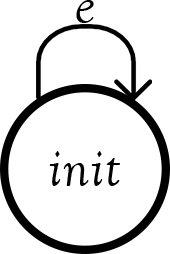
\includegraphics{null}\end{center}
  \item for \(\epsilon\), we have \(M = (\{init\},\ \Sigma^e,\
    \delta,\ init,\ \{init\})\) and graphically \begin{center}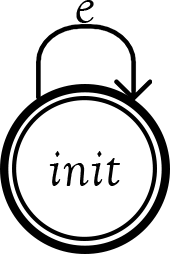
\includegraphics{epsilon}\end{center}
  \item for \(a\), we have \(M = (\{init, accept\},\ \Sigma^e,\
    \delta,\ init,\ \{accept\})\) and graphically \begin{center}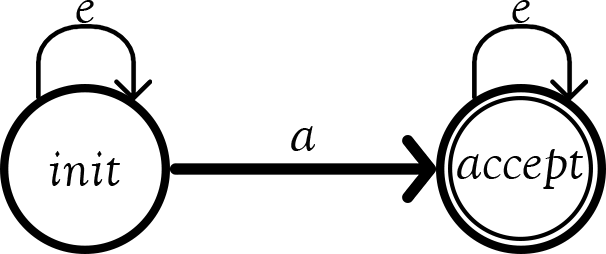
\includegraphics{singleton}\end{center}
  \item if \(N_1 = (Q_1,\ \delta_1,\ q_{01},\ F_1)\) and \(N_2 =
    (Q_2,\ \delta_2,\ q_{02},\ F_2)\) are \(\epsilon\)-NFAs translated from the
    regular expressions \(e_1\) and \(e_2\) respectively, then
    \begin{enumerate}[nolistsep]
      \item for \((e_1\ |\ e_2)\), we have \(M = (\{init\} \cup Q_1
        \cup Q_2,\ \Sigma^e,\ \delta,\ init,\ F_1 \cup F_2)\) and
        graphically \begin{center}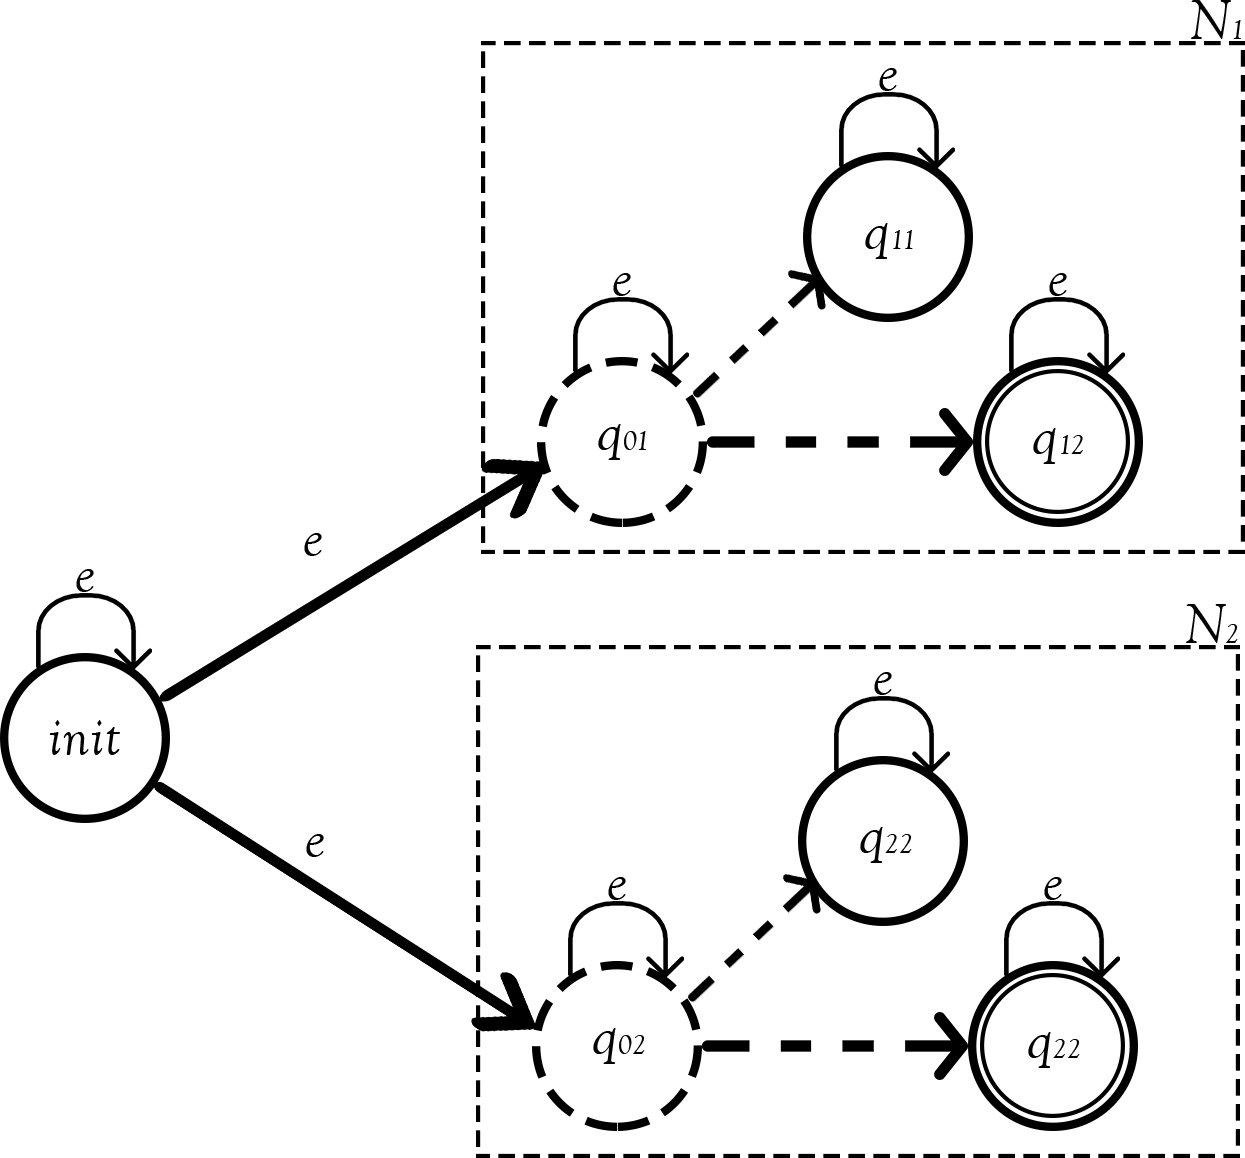
\includegraphics{union}\end{center}
      \item for \(e_1\cdot e_2\), we have \(M = (Q_1 \cup \{mid\}
        \cup Q_2,\ \Sigma^e,\ \delta,\ init,\ F_2)\) and graphically \begin{center}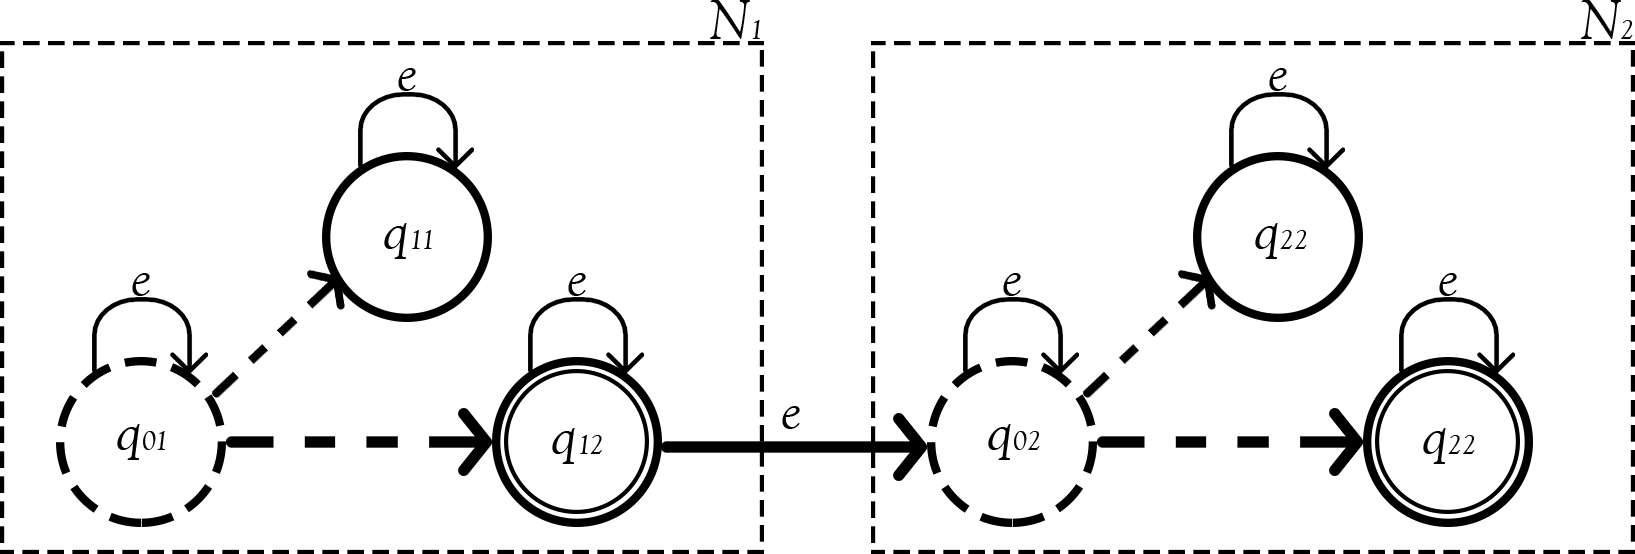
\includegraphics{concat}\end{center}
      \item for \(e_1^{\ *}\), we have \(M = (\{init\} \cup Q_1,\
        \Sigma^e,\ \delta,\ init,\ \{init\} \cup F_1)\) and
        graphically \begin{center}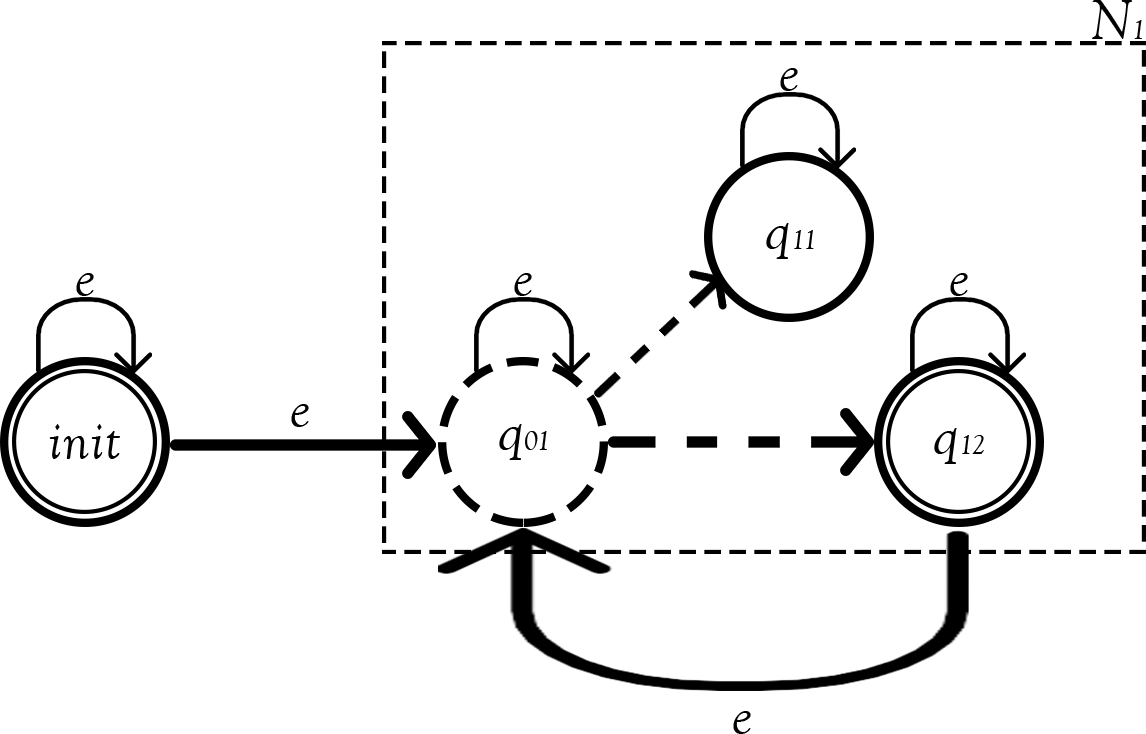
\includegraphics{star}\end{center}
     \end{enumerate}
\end{enumerate}


\paragraph{Theorem 1.1} For any given regular expressions, its accepted
language is equal to the language accepted by its translated
\(\epsilon\)-NFA using Thompson's Construction. i.e. \(L(e) =
L(translted\ \epsilon\)-NFA\()\). 

\paragraph{Proof 1.1} We have to prove that for any regular expressions \(e\), \(L(e) \subseteq
L(translated\ \epsilon\)-\(NFA)\) and \(L(e) \supseteq L(translated\
\epsilon\)-\(NFA)\) by induction on \(e\). 

\subparagraph{Base cases} For \(\O\), \(\epsilon\) and \(a\), by Definition 5.1, it is obvious that the
language accepted by them are equal to the language accepted by their
translated \(\epsilon\)-NFA. 

\subparagraph{Induction hypothesis} For any regular expressions
\(e_1\) and \(e_2\), let \(N_1 =
(Q_1,\ \delta_1,\ q_{01},\ F_1)\) and \(N_2 = (Q_2,\ \delta_2,\
q_{02},\ F_2)\) be their translated \(\epsilon\)-NFA using Definition
5.1 respectively. Then we assume that \(L(e_1) = L(N_1)\) and \(L(e_2) =
L(N_2)\). 
\\
\par \textbf{Inductive steps}
\par 1) For \((e_1\ |\ e_2)\), let \(M = (Q,\ \delta,\ q_0,\ F) = (\{init\} \cup Q_1 \cup Q_2,\
\delta,\ init,\ F_1 \cup F_2)\) be its translated \(\epsilon\)-NFA
using Definition 5.1. Then for any string \(w\), 

\par 1.1) if \((e_1\ |\ e_2)\) accepts \(w\), by Definition 3.2,
either i) \(e_1\) accepts \(w\) or ii) \(e_2\) accepts \(w\). Assuming case i), then by
induction hypothesis, \(N_1\) also accepts \(w\) which also implies
that there exists a chain \((q_{01} , w^e) \vdash^* (q , \epsilon)\) in \(N_1\) such that
\(w^e\) is an \(\epsilon\)-string of \(w\) and \(q \in F_1\). Now, we can
add an \(\epsilon\)-transition from \(init\) to \(q_{01}\) in \(M\)
such that \((init , \epsilon w^e) \vdash^* (q , \epsilon)\)
because \(q_{01} \in \delta\ init\ \epsilon\). Now, since \(q \in
F_1\) implies that \(q \in F\) and \(\epsilon w^e\)
is also an \(\epsilon\)-string of \(w\); therefore \(w \in L(M)\). The same argument also applies
for the case when \(e_2\) accepts \(w\). Since we have proved that \(w \in L(e_1\ |\ e_2)
\Rightarrow w \in L(M)\); therefore \(L(e_1\ |\ e_2) \subseteq L(M)\)
also follows;

\par 1.2) if \(M\) accepts \(w\), then there must exists a chain \((init , w^e) \vdash^* (q ,
\epsilon)\) in \(M\) such that \(w^e\) is an \(\epsilon\)-string of \(w\) and \(q
\in F\). Since \(q \in F\), therefore \(q \neq init\). By Definition
5.1, there are only two possible ways for \(init\) to reach \(q\), via \(q_{01}\) or ii) 
\(q_{02}\). Assuming case i), then we have \((init , \epsilon^+w_1) \vdash^*
(q_{01} , w_1)\) and \((q_{01} , w_1) \vdash^* (q , \epsilon)\) where \(w^e =
\epsilon^+w_1\) and \(q \in Q_1\). Since we have \(q \in F\) and \(q \in
Q_1\); therefore we have \(q \in F_1\). Also \(w_1\) is also an
\(\epsilon\)-string of \(w\), thus the chain \((q_{01} , w_1) \vdash^* (q , \epsilon)\)
implies that \(w \in L(N_1)\). By induction hypothesis, we have \(w \in L(e_1)\) and thus \(w \in L(e_1\
|\ e_2)\). The same argument also applies for case ii). Since we have
proved that \(w \in
L(M) \Rightarrow w \in L(e_1\ |\ e_2)\); therefore \(L(e_1\ |\ e_2)
\supseteq L(M)\) also follows;

\par 1.3) combining 1.1  and 1.2, we have \(L(e_1\ |\ e_2) = L(M)\). 
\\
\par 2) For \((e_1 \cdot e_2)\), let \(M = (Q,\ \delta,\ q_0,\ F) = (Q_1 \cup \{mid\} \cup Q_2,\ \delta,\ q_{01},\ F_2)\) be its
translated \(\epsilon\)-NFA using Definition 5.1. Then for any string
\(w\), 

\par 2.1) if \((e_1 \cdot e_2)\) accepts \(w\), then by Definition
3.2, there exists a \(u \in L(e_1)\) and a \(v \in L(e_2)\) such that \(w
= uv\). By induction hypothesis, \(u \in L(e_1)\) implies that \(u \in
L(N_1)\) and \(v \in L(e_2)\) implies that \(v \in L(N_2)\). So there
exists a chain: i)\((q_{01} ,
u^e) \vdash^* (q_1 , \epsilon)\) in \(N_1\) where
\(u^e\) is an \(\epsilon\)-string of \(u\) and \(q_1 \in F_1\) and
ii) \((q_{02} , v^e) \vdash^* (q_2 , \epsilon)\) in \(N_2\)
where \(v^e\) is an \(\epsilon\)-string of \(v\) and \(q_2 \in
F_2\). Now we can add an \(\epsilon\)-transition from \(q_1\) to \(mid\) and
from \(mid\) to \(q_{02}\) in order to construct a chain in
\(M\). Since\(q_2
\in F_2\) implies that \(q_2 \in F\) and \(u^ev^e\) is an
\(\epsilon\)-string of \(w\) implies that so is \(u^e\epsilon \epsilon
v^e\); therefore \(w \in L(M)\). Since we have proved that \(w \in
L(e_1 \cdot e_2) \Rightarrow w \in L(M)\), therefore \(L(e_1 \cdot
e_2) \subseteq L(M)\) also follows;

\par 2.2) if \(M\) accepts \(w\), then by Definition 5.1, there must exists
a chain \((init , w^e) \vdash^* (q , \epsilon)\) in \(M\) where
\(w^e\) is an \(\epsilon\)-string of \(w\) and \(q \in F\). Since \(q
\in F\), so \(q\) must also be in \(Q_2\). The only possible way for
\(q_{01}\) to reach \(q\) is to go through \(mid\). This implies that
there exists a \(q_1 \in Q_1\), a \(u^e \in \Sigma^{e*}\) and a \(v^e \in
\Sigma^{e*}\) such that \((q_{01} , u^e\epsilon^+ \epsilon^+ v^e) \vdash^*
(q_1 , \epsilon^+ \epsilon^+ v^e)\), \(q_1 \in F_1\), \((q_{02} , v^e)
\vdash^* (q_2 , \epsilon)\) and \(w^e = u^e\epsilon^+ \epsilon^+
v^e\). Let \(u\) and \(v\) be the strings represented by \(u^e\) and
\(v^e\) respectively, we have \(u \in L(N_1)\) and \(v \in
L(N_2)\). Then, by induction hypothesis, \(u \in L(e_1)\) and \(v \in
L(e_2)\). Since \(w^e\) is an \(\epsilon\)-string of \(w\), so is
\(u^ev^e\) and thus \(w =
uv\). From this, we can deduce that \(w \in L(e_1 \cdot e_2)\). Since
we have proved that \(w \in L(M) \Rightarrow w \in L(e_1 \cdot e_2)\),
therefore \(L(e_1 \cdot e_2) \supseteq L(M)\) also follows;

\par 2.3) combining 2.1 and 2.2, we have \(L(e_1 \cdot e_2) = L(M)\). 
\\
\par 3) For \(e^*\), let \(M = (Q,\ \delta,\ q_0,\ F) = (Q_1 \cup \{mid\} \cup Q_2,\ \delta,\ q_{01},\ F_2)\) be its
translated \(\epsilon\)-NFA using Definition 5.1. Then for any string
\(w\), 

\par 3.1) if \((e^*)\) accepts w, then there must exists a number
\(n\) such that \(w \in (L\) \^\ \(n)\). Now, lets do induction on
\(n\). \textbf{Base case:} when \(n = 0\), \(L\) \^\ \(0 = \) ...

\par 3.2) if \(M\) accepts \(w\), ... 

\par 3.3) combining 3.1 and 3.2, we have \(L(e_1^*) =
L(M)\). \(\Box\)

\subsection{Non-deterministic Finite Automata}

\paragraph{Definition 6.1} A NFA is a 5-tuple \(M = (Q
,\ \Sigma,\ \delta,\ q_0,\ F)\), where
\begin{enumerate}[nolistsep]
  \item \(Q\) is a finite set of states;
  \item \(\Sigma\) is the set of alphabets;
  \item \(\delta\) is a mapping from \(Q \times\ \Sigma\) to
    \(\mathcal P \left({Q}\right)\) which defines the behaviour of the automata;
  \item \(q_0\) in \(Q\) is the initial state;
  \item \(F \subseteq Q\) is the set of accepting states. 
\end{enumerate}
\vspace{0.7pc}
\begin{lstlisting}[caption=NFA,mathescape=true]
record NFA : Set$_1$ where
  field
    Q      : Set
    $\delta$       : Q $\to$ $\Sigma$ $\to$ DecSubset Q
    q$_0$      : Q
    F      : DecSubset Q
    Q?     : DecEq Q
    |Q|-1  : $\mathbb{N}$
    It     : Vec Q (suc |Q|-1)
    $\forall$q$\in$It    : (q : Q) $\to$ (q $\in^V$ It)
    unique : Unique It
\end{lstlisting}
%\vspace{1pc}
\paragraph{} The set of alphabets \(\Sigma : Set\) is passed to the file
parameters. Together with \(Q\), \(\delta\),
\(q_0\) and \(F\), these five fields correspond to the 5-tuple
\(\epsilon\)-NFA. \(Q?\) is
the decidable equality of \(Q\). \(|Q|-1\) is the number of states -
1. '\(It\)' is a vector of length \(|Q|\) containing all the
states in \(Q\). \(\forall q\in It\) is a
proof that all states in \(Q\) are also in the vector
'\(It\)'. \(unique\) is a proof that there is no repeating elements in
'\(It\)'. These extra fields are important when computing
\(\epsilon\)-closures, we will look into them again later in more
details.  

\paragraph{} Now, we want to define the set of strings \(\Sigma^*\) accepted by a given
NFA. However, before we can do this, we have to define
some operations.

\paragraph{Definition 6.2} A configuration is a pair \(Q \times
\Sigma^*\). 

\paragraph{Definition 6.3} A move by an \(\epsilon\)-NFA \(N\) is
represented by a binary function \(\vdash\) on configurations. We say
that \((q, aw) \vdash (q' , w)\) for all w in \(\Sigma^*\)
if and only if \(q' \in \delta (q , a)\) where \(a \in \Sigma\). 

\begin{lstlisting}[mathescape=true]
  _$\vdash$_ : (Q $\times$ $\Sigma$ $\times$ $\Sigma^*$) $\to$ (Q $\times$ $\Sigma^*$) $\to$ Set
  (q , a , w) $\vdash$ (q' , w') = w $\equiv$ w' $\times$ q' $\in^d$ $\delta$ q a
\end{lstlisting}

\paragraph{Definition 6.4} We say that \(C \vdash^0 C'\) if and only
if \(C = C'\). We say that \(C_0 \vdash^k C_k\) for any \(k \geq 1\) if and only if there exists a chain of
configurations \(C_1, C_2, ..., C_{k-1}\) such that \(C_i \vdash
C_{i+1}\) for all \(0 \leq i \leq k\). 

\begin{lstlisting}[mathescape=true]
  _$\vdash^k$_-_ : (Q $\times$ $\Sigma^*$) $\to$ $\mathbb{N}$ $\to$ (Q $\times$ $\Sigma^*$) $\to$ Set
  (q , w) $\vdash^k$ zero  - (q' , w')
    = q $\equiv$ q' $\times$ w $\equiv$ w'
  (q , w) $\vdash^k$ suc n - (q' , w') 
    = $\exists$[ p $\in$ Q ] $\exists$[ a $\in$ $\Sigma$ ] $\exists$[ u $\in$ $\Sigma^*$ ]
      (w $\equiv$ a :: u $\times$ (q , a , u) $\vdash$ (p , u) $\times$ (p , u) $\vdash^k$ n - (q' , w'))
\end{lstlisting}

\paragraph{Definition 6.5} We say that \(C \vdash^* C'\) if and only
if there exists a number of chains \(n\) such that \(C \vdash^n C'\). 

\begin{lstlisting}[mathescape=true]
  _$\vdash^*$_ : (Q $\times$ $\Sigma^*$) $\to$ (Q $\times$ $\Sigma^*$) $\to$ Set
  (q , w) $\vdash^*$ (q' , w') = $\exists$[ n $\in$ $\mathbb{N}$ ] (q , w) $\vdash^k$ n - (q' , w')
\end{lstlisting}

\paragraph{Definition 6.6} For any string \(w\), it is accepted by an NFA \(N\)
if and only if there exists a chain of configurations from \(q_0 ,
w)\) to \(q , \epsilon\) where \(q \in F\). 

\paragraph{Definition 6.7} The language accepted by an
NFA is given by the set \(\{\ w\ |\ \exists q\in F.\ (q_0\ ,\
w) \vdash^* (q\ ,\ \epsilon)\ \}\). 

\begin{lstlisting}[mathescape=true]
  L$^N$ : NFA $\to$ Language
  L$^N$ nfa = $\lambda$ w $\to$ $\exists$[ q $\in$ Q ] (q $\in^d$ F $\times$ (q$_0$ , w) $\vdash^*$ (q , []))
\end{lstlisting} 

\subsection{Removing \(\epsilon\)-transitions}
\paragraph{} ...

\subsection{Deterministic Finite Automata}
\paragraph{} ...

\subsection{Powerset Construction}
\paragraph{} ...

\subsection{Minimal DFA}
\paragraph{} ...

\subsection{Minimising DFA}
\paragraph{} ...

\newpage
\section{Further Extensions}
\par Myhill-Nerode Theorem, Pumping Lemma

\newpage
\section{Evaluation}

\subsection{Correctness and Readability}
\paragraph{} According to \cite{geuvers2009}, proofs have two major roles: 1)
to convince the readers that the statement is correct and 2) to expain
why the statement is correct. The first part is consist of the
verification of small individual reasoning steps. We have to
determines if these steps constitute a correct proof. The second part
requires the proof to be able to give an intuition of the
statement. In the paragraphs below, we will evaluate the project based
on these two criteria. 

\paragraph{Correctness} In the traditional way, when a mathematician
submits the proof of his/her concepts, a group of mathematicians will
evaluate it and see if the proof is correct or not. Alternatively, if we
formalise the proof in a proof assistant, the proof will be checked
automatically by the compiler. The only difference is that we are now
relying on the compiler and the machine that it runs on rather
than a group of mathematicians. Therefore, if the compiler and the
machine works properly, then any formalised proof that
can be compiled without errors are said to be correct. In our case, we
have the type checker and termination checker in Agda to serve the
purpose. Another aspect is that the correctness of a proof should be
obtained by verifiying the individual small reasoning steps within the
proof. When writing proofs in paper, we usually omit the proofs of
some obvious theorem such as the associativity of addition. However,
in Agda, we have to make explicit all the proofs for every lemma and
theorem. Therefore, the correctness of a Agda proof will always depend on the
correctness of the smaller proofs that it contains. We can conclude
that a computer proof is a very convincing argument. 

\paragraph{Readability} The other purpose of a proof is to explain why
a certain statement is correct. 


\subsection{Different Choices of Representaion}
\paragraph{} Apart from the two criteria, the other important aspect
is the way that a proof is formalised. When
writing proofs in papers, we are not usually required to provide
concreate representations for abstract mathematical objects like
subsets. However, when writing proofs in Type Theory, we usually have to provide a
representation for them. The consequence is that different forms of represenation
will lead to different formalisations and thus contributes to the
easiness/difficulty in writing the proofs. In the following part, we
will discuss different representations we have choosen and their
effect. 

\paragraph{The set of states (\(Q\)) in an automata} In our approach,
we used \(Q : Set\) to represent the set of states while in
\cite{firsov2013}, they used vector as the representation. The 


\paragraph{Subset and DecidableSubset} ...


\newpage
\section{Discussion}
\paragraph{} If start over ... ?

\paragraph{} Is it feasible to write computer proof in practice?

\newpage
\section{Conclusion}
\paragraph{} Recap what is done

\newpage
\section*{References}
\addcontentsline{toc}{section}{References}
\bibliographystyle{plain}
\bibliography{references}

\newpage
\section*{Appendices}
\addcontentsline{toc}{section}{Appendices}
\paragraph{} Agda Code?

\end{document}